\documentclass[tikz,border=12pt]{standalone}
\usepackage[T1]{fontenc}
\usepackage{mathpazo}
\usepackage{amsmath,amssymb}
\usetikzlibrary{arrows.meta, positioning, calc, fit, patterns, decorations.pathreplacing}

\definecolor{stblue}{HTML}{7B97AD}
\definecolor{rwgold}{HTML}{B8995E}
\definecolor{sage}{HTML}{7A9A7E}
\definecolor{dkbrown}{HTML}{3D3530}
\definecolor{wmgray}{HTML}{7B7067}
\definecolor{cream}{HTML}{F9F6F0}
\definecolor{border}{HTML}{D4C9B8}
\definecolor{terracotta}{HTML}{C47A6A}
\definecolor{lavender}{HTML}{907EA0}

\begin{document}
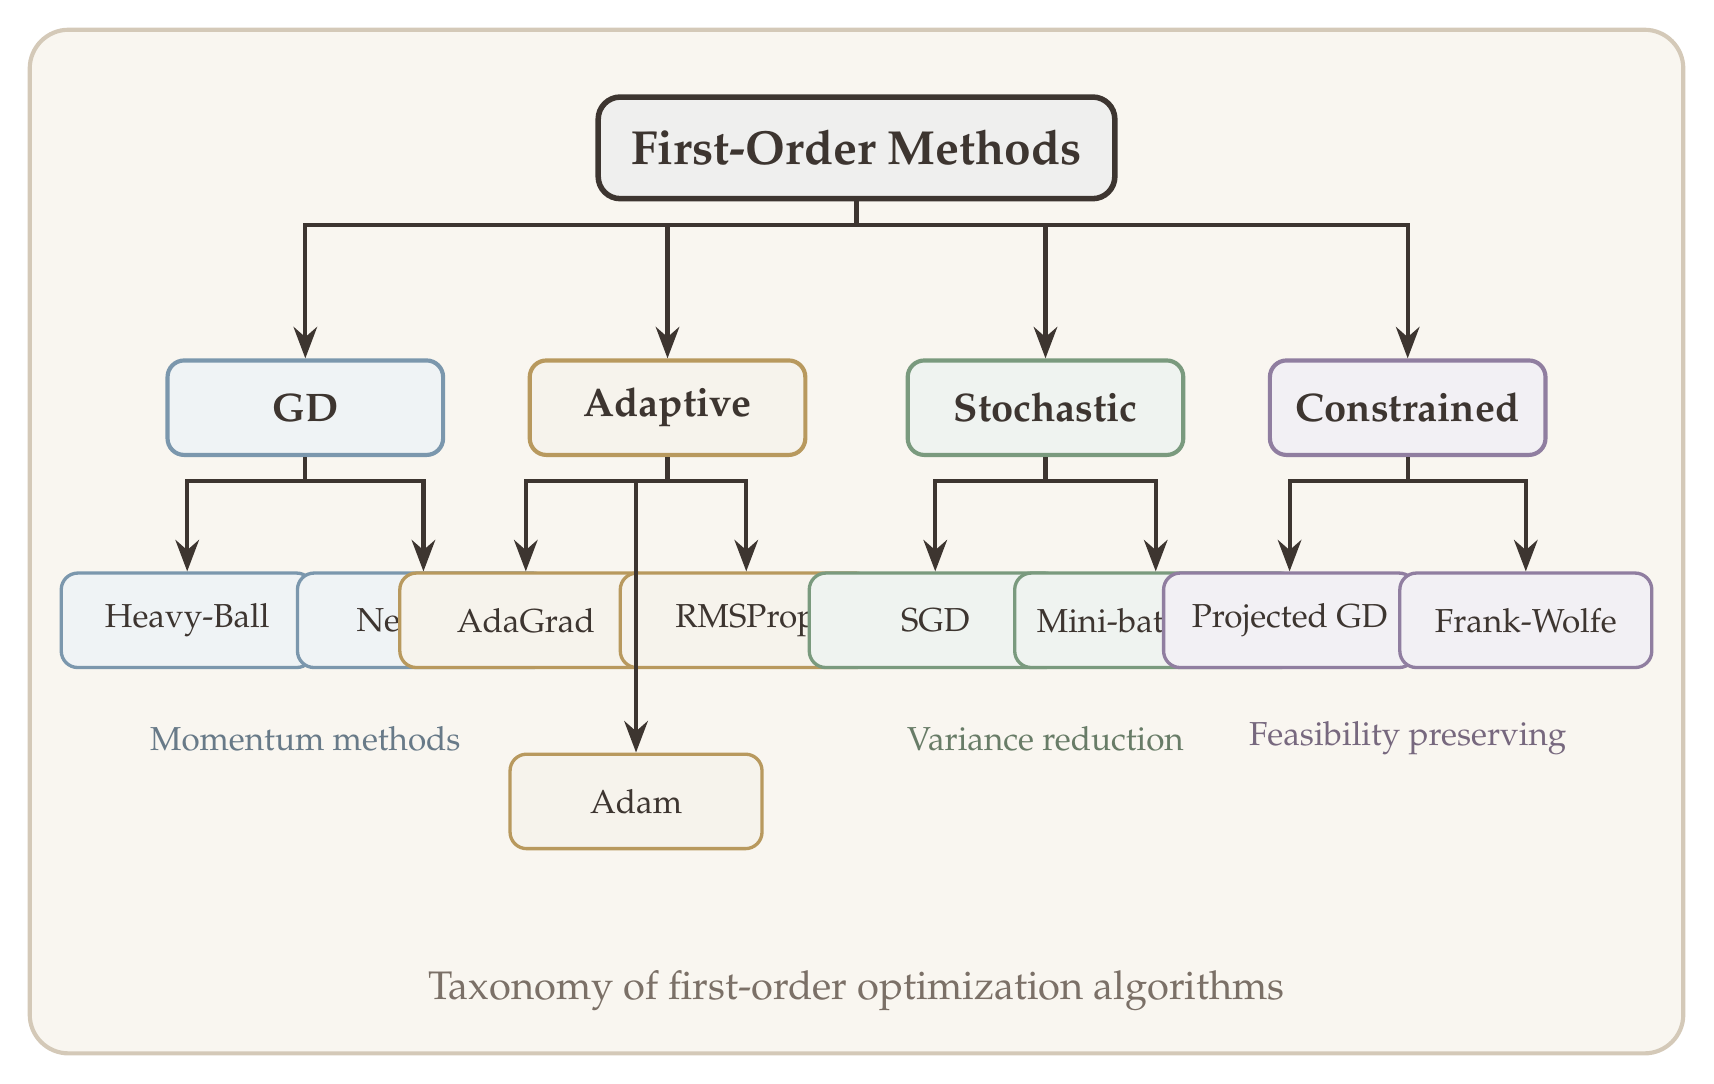
\begin{tikzpicture}[>={Stealth[length=4mm, width=3mm]}, line width=1.5pt,
  rootbox/.style={fill=dkbrown!8, draw=dkbrown, line width=2pt, rounded corners=8pt,
                  font=\LARGE\bfseries, text=dkbrown, inner sep=12pt, minimum width=5.5cm},
  branchbox/.style={fill=#1!12, draw=#1, line width=1.5pt, rounded corners=6pt,
                    font=\Large\bfseries, text=dkbrown, inner sep=8pt, minimum width=3.5cm,
                    minimum height=1.2cm},
  leafbox/.style={fill=#1!12, draw=#1, line width=1.2pt, rounded corners=6pt,
                  font=\large, text=dkbrown, inner sep=8pt, minimum width=3.2cm,
                  minimum height=1.2cm},
  conn/.style={dkbrown, line width=1.5pt, ->}
]

% Background
\fill[cream, rounded corners=14pt] (-10.5,-9) rectangle (10.5,4);
\draw[border, line width=1.5pt, rounded corners=14pt] (-10.5,-9) rectangle (10.5,4);

% Root
\node[rootbox] (root) at (0,2.5) {First-Order Methods};

% Branch nodes
\node[branchbox=stblue] (gd) at (-7,-0.8) {GD};
\node[branchbox=rwgold] (adaptive) at (-2.4,-0.8) {Adaptive};
\node[branchbox=sage] (stochastic) at (2.4,-0.8) {Stochastic};
\node[branchbox=lavender] (constrained) at (7,-0.8) {Constrained};

% Connections from root
\draw[conn] (root.south) -- ++(0,-0.3) -| (gd.north);
\draw[conn] (root.south) -- ++(0,-0.3) -| (adaptive.north);
\draw[conn] (root.south) -- ++(0,-0.3) -| (stochastic.north);
\draw[conn] (root.south) -- ++(0,-0.3) -| (constrained.north);

% GD leaves
\node[leafbox=stblue] (hb) at (-8.5,-3.5) {Heavy-Ball};
\node[leafbox=stblue] (nes) at (-5.5,-3.5) {Nesterov};
\draw[conn] (gd.south) -- ++(0,-0.3) -| (hb.north);
\draw[conn] (gd.south) -- ++(0,-0.3) -| (nes.north);

% Adaptive leaves
\node[leafbox=rwgold] (adagrad) at (-4.2,-3.5) {AdaGrad};
\node[leafbox=rwgold] (rmsprop) at (-1.4,-3.5) {RMSProp};
\node[leafbox=rwgold] (adam) at (-2.8,-5.8) {Adam};
\draw[conn] (adaptive.south) -- ++(0,-0.3) -| (adagrad.north);
\draw[conn] (adaptive.south) -- ++(0,-0.3) -| (rmsprop.north);
\draw[conn] (adaptive.south) -- ++(0,-0.3) -| (adam.north);

% Stochastic leaves
\node[leafbox=sage] (sgd) at (1.0,-3.5) {SGD};
\node[leafbox=sage] (minibatch) at (3.8,-3.5) {Mini-batch SGD};
\draw[conn] (stochastic.south) -- ++(0,-0.3) -| (sgd.north);
\draw[conn] (stochastic.south) -- ++(0,-0.3) -| (minibatch.north);

% Constrained leaves
\node[leafbox=lavender] (pgd) at (5.5,-3.5) {Projected GD};
\node[leafbox=lavender] (fw) at (8.5,-3.5) {Frank-Wolfe};
\draw[conn] (constrained.south) -- ++(0,-0.3) -| (pgd.north);
\draw[conn] (constrained.south) -- ++(0,-0.3) -| (fw.north);

% Convergence rate annotations at bottom
\node[font=\large, text=stblue!70!dkbrown] at (-7,-5.0) {Momentum methods};
\node[font=\large, text=sage!70!dkbrown] at (2.4,-5.0) {Variance reduction};
\node[font=\large, text=lavender!70!dkbrown] at (7,-5.0) {Feasibility preserving};

% Bottom note
\node[font=\Large, text=wmgray] at (0,-8.2) {Taxonomy of first-order optimization algorithms};

\end{tikzpicture}
\end{document}
